\documentclass[../../main.tex]{subfiles}

\begin{document}

Mithilfe der Überlegungen zu Äquivalenzumformungen, die wir bisher angestellt haben, haben wir eine solide Grundlage, um zu unserer eigentlichen Fragestellung zurückzukehren, nämlich der, wie wir systematisch lineare Gleichungen lösen können. Um damit loszulegen, sollten wir zunächst festlegen, was genau denn nun eine lineare Gleichung ist.

Im Wesentlichen kann man sich lineare Gleichungen so vorstellen, dass sie eine Darstellung von Balkenwaagen sind: Auf jeder Seite einer linearen Gleichung erlauben wir die Summe von Gegenständen, die wir auf eine Waagschale legen könnten. Das waren bei uns:
\begin{itemize}
    \item Kugeln mit dem Gewicht $x$
    \item Gewichte mit beliebigen Zahlenwerten
\end{itemize}

Jede Seite einer Waagschale kann durch einen Term der Form $ax+b$ dargestellt werden, wobei $a$ die Anzahl der Kugeln und $b$ die Summe der Gewichte ist. Sind beispielsweise $5$ Kugeln sowie Gewichte mit einer Summe von 12 auf der Waage, so ist das Gesamtgewicht in der Waagschale $5x+12$.

Auch wenn mit Balkenwaagen eine negative Anzahl von Kugeln, Bruchteile von Kugeln oder negative Gewichte nicht funktionieren, wollen wir alle Gleichungen als linear bezeichnen, bei denen die linke und die rechte Seite jeweils die Form $ax+b$ mit beliebigen $a,b\in\Real$ haben. Das ist der Punkt, an dem unsere Vorstellung mit der Waage nicht mehr besonders gut funktioniert. Im Wesentlichen sind das immer noch genau die Gleichungen, die sich (bis auf ein paar kleine Probleme) auf Waagen darstellen lassen.

\begin{center}
    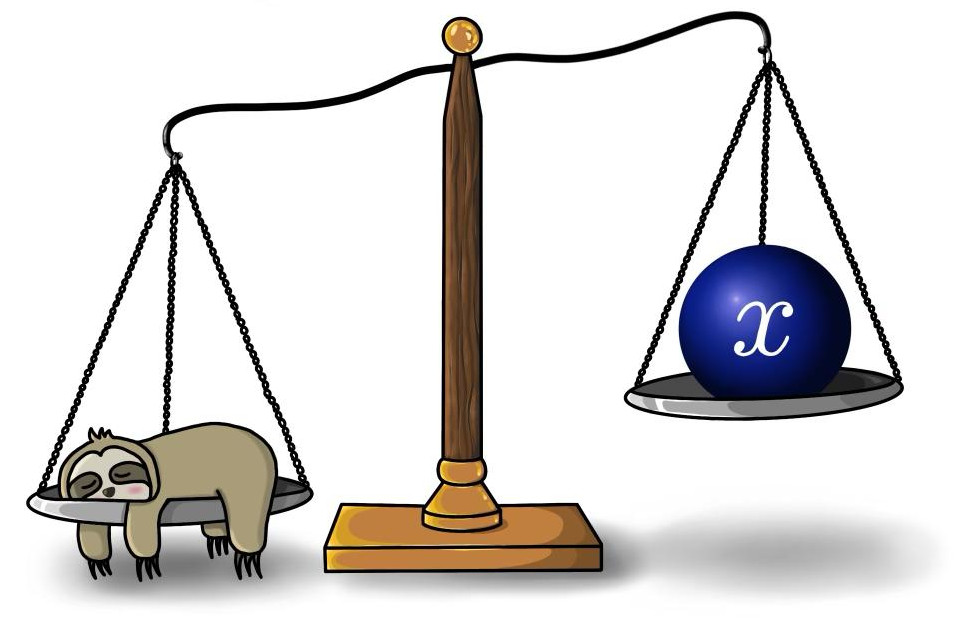
\includegraphics[height=4.6cm]{images/faultier-balkenwaage.jpg}
\end{center}
\vfill

\begin{example}{}
    Die Gleichung 
    \[7x+5=2x\] 
    ist eine lineare Gleichung. Die linke Seite ist hier eine Darstellung von \enquote{7 Kugeln und Gewichte mit dem Wert 5} und die rechte Seite beschreibt \enquote{zwei Kugeln}. Oder, etwas technischer: Die linke Seite hat die Form $ax+b$, wenn man $a=7$ und $b=5$ wählt. Die rechte Seite hat diese Form ebenfalls, und zwar mit $a=2$ und $b=0$.
\end{example}

\begin{example}{}
    Auch die Gleichung 
    \[5(x+4)=2\cdot (3+x)-8\] 
    ist eine lineare Gleichung. Sie sieht zwar erstmal merkwürdig aus, aber beide Seiten lassen sich in die Form $ax+b$ umstellen. Auf der linken Seite steht $5(x+4)$. Das lässt sich umformen zu $5x+20$ (und damit haben wir wieder die Form $ax+b$). Auf der rechten Seite steht 
    \[2\cdot (3+x)-8=6+2x-8=2x-2\] 
    (und mit $2x-2$ haben wir wieder die Form $ax+b$). Deshalb ist auch die Gleichung $5(x+4)=2\cdot (3+x)-8$ linear.
\end{example}

\begin{example}{}
    Die Gleichung 
    \[2^x+5=0\] 
    ist nicht linear: Wir können sie nicht so umformen, dass links $ax+b$ steht, weil wir die Potenz nicht loswerden können. Aus demselben Grund ist auch 
    \[x^2-4x+9=0\] 
    keine lineare Gleichung, denn $x^2$ lässt sich nicht ohne weiteres eliminieren.
\end{example}

\begin{definition}{Lineare Gleichung}
    Eine \textbf{lineare Gleichung} ist eine Gleichung, deren Seiten durch Termumformung in die Form $ax+b$ mit $a,b\in\Real$ gebracht werden können.
\end{definition}

Um zu überlegen, wie wir lineare Gleichungen auflösen können, kehren wir trotzdem noch einmal zu unserer Anschauung als Waagen zurück. 
Uns können also beliebige Gleichungen begegnen, auf deren linker und rechter Seite beliebig viele Kugeln und Gewichte liegen. Das Ziel 
ist es, $x$ (bzw. eine Kugel) zu isolieren, sodass auf der anderen Seite kein $x$ mehr steht.

Wir überlegen uns dafür verschiedene Zwischenziele und es wird schnell deutlich werden, dass wir diese bei jeder linearen Gleichung 
auf eine ähnliche Weise erreichen können. Um besser zu zeigen, \emph{warum} wir gewisse Umformungen vornehmen, wird das Verfahren 
hier rückwärts präsentiert. Wir zeigen die verschiedenen Zwischenziele, um die Lösungsmenge einer beliebigen linearen Gleichung zu finden.

\label{lineare-gleichungen-loesungsverfahren}
\textbf{Zwischenziel 4: Fertig aufgelöste Gleichung}
\parpic[r]{
    \begin{linearEquation}
        %Füllung linke Waagschale
        \node[white,marble,inner sep=.12cm] at (-1,0.35) {$x$};
        %Füllung rechte Waagschale
        \fill (0.75,0.25) -- (1.25,0.25) -- (1.2,0.65) -- (0.8,0.65) -- cycle;
        \draw[line width=0.75mm] (1,0.71) circle[radius=0.06cm];
        \node[white] at (1,0.45) {$23$};
    \end{linearEquation}
}

Am einfachsten ist es natürlich, wenn wir schon am Ziel sind und eine fertig aufgelöste Gleichung haben: 
\[x=\langle \text{Zahl} \rangle.\]
Die Gleichung $x=23$ ist bereits fertig aufgelöst. Wir müssen nur noch die \textbf{Lösungsmenge} $\Solutions=\{23\}$ \textbf{ablesen} und sind fertig.

\textbf{Zwischenziel 3: Kugeln links, Gewichte rechts}

\parpic[r]{
    \begin{linearEquation}
        %Füllung linke Waagschale
        \node[white,marble,inner sep=.12cm] at (-1.15,0.35) {$x$};
        \node[white,marble,inner sep=.12cm] at (-0.85,0.35) {$x$};
        %Füllung rechte Waagschale
        \fill (0.75,0.25) -- (1.25,0.25) -- (1.2,0.65) -- (0.8,0.65) -- cycle;
        \draw[line width=0.75mm] (1,0.71) circle[radius=0.06cm];
        \node[white] at (1,0.45) {$46$};
    \end{linearEquation}
}

Wenn entgegen unseres vorher formulierten Ziels nicht nur eine Kugel, sondern eine beliebige Anzahl an Kugeln auf der linken Seite liegen, dann sieht die Gleichung folgendermaßen aus:
\[ax=\langle \text{Zahl} \rangle.\]
Um von hier aus schnell Zwischenschritt 4 zu erreichen, können wir die Gleichung durch die Anzahl der Kugeln auf der linken Seite dividieren. In der abgebildeten Gleichung $2x=46$ teilen wir die Gleichung also durch $2$. Dadurch behalten wir rechts nach wie vor eine Zahl (die nicht mehr das Gewicht von zwei Kugeln, sondern das Gewicht einer einzelnen Kugel angibt), allerdings haben wir links nur noch eine einzige Kugel und sind somit beim Zwischenziel 4 angekommen.

Wir \textbf{teilen} eine Gleichung der obigen Gestalt also \textbf{durch den Vorfaktor von \emph{x}} (also durch $a$) und gelangen sofort zu Zwischenziel 4.

\vbox{
\textbf{Zwischenziel 2: Zusammengefasste Gleichung ohne Klammern}

\parpic[r]{
    \begin{linearEquation}
        %Füllung linke Waagschale
        \fill (-0.85,0.25) -- (-0.45,0.25) -- (-0.5,0.6) -- (-0.8,0.6) -- cycle;
        \draw[line width=0.75mm] (-0.65,0.66) circle[radius=0.06cm];
        \node[white] at (-0.65,0.42) {$5$};
        \node[white,marble,inner sep=.12cm] at (-1,0.35) {$x$};
        \node[white,marble,inner sep=.12cm] at (-1.2,0.35) {$x$};
        \node[white,marble,inner sep=.12cm] at (-1.4,0.35) {$x$};
        %Füllung rechte Waagschale
        \fill (0.65,0.25) -- (1.15,0.25) -- (1.1,0.65) -- (0.7,0.65) -- cycle;
        \draw[line width=0.75mm] (0.9,0.71) circle[radius=0.06cm];
        \node[white] at (0.9,0.45) {$51$};
        \node[white,marble,inner sep=.12cm] at (1.3,0.35) {$x$};
    \end{linearEquation}
}

In diesem Schritt gehen wir von einer beliebigen Gleichung
\[ax+b=cx+d\]
mit Zahlen $a,b,c,d\in\Real$ aus. Um das nächste Zwischenziel zu erreichen, müssen alle Kugeln links und alle Gewichte rechts liegen. Wir müssen im Beispiel $3x+5=51+x$ also zwei Dinge tun:
\picskip{0}
\begin{itemize}
    \item Auf der rechten Seite alle Kugeln entfernen (und genauso viele Kugeln auch von der linken Seite entfernen)
    \item Auf der linken Seite alle Gewichte entfernen (und genauso viele Gewichte auch von der rechten Seite entfernen)
\end{itemize}
Anschließend sind links keine Gewichte und rechts keine Kugeln mehr übrig, das heißt, wir haben Zwischenziel 3 erreicht. In der Gleichung $3x+5=51+x$ stört auf der linken Seite die $5$. Wir subtrahieren auf beiden Seiten $5$ und erhalten die Gleichung $3x=46+x$. Nun muss noch das störende $x$ auf der rechten Seite entfernt werden. Wir subtrahieren $x$ auf beiden Seiten und erhalten die Gleichung $2x=46$.

\textbf{Zwischenziel 1: Beliebige lineare Gleichung}

Mit diesem Zwischenziel starten wir eigentlich immer automatisch (außer wir müssen von einem Sachzusammenhang ausgehend erst noch eine Gleichung aufstellen). Bevor die Gleichung aufgelöst werden kann, sollte sie vereinfacht werden. Dazu werden alle Klammern durch \textbf{Ausmultiplizieren} aufgelöst und gleichartige \textbf{Terme zusammengefasst}.

Zum Beispiel kann die Gleichung $2(x+2)+x+1=17(x+3)-16x$ noch deutlich vereinfacht werden. Wir lösen zunächst die Klammern auf und erhalten
\[\colorbrace{2x+4}{\text{Klammer}}+x+1=\colorbrace{17x+51}{\text{Klammer}}-16x.\]
Schließlich fassen wir die Terme zusammen zu $3x+5=x+51$ und haben Zwischenziel 2 erreicht.

Mit diesen Schritten lässt sich jede lineare Gleichung auflösen. Wenn du also eine Aufgabe mit einer linearen Gleichung auflösen musst, dann ist deine Aufgabe, nach einander die verschiedenen Zwischenziele zu erreichen. Daraus ergeben sich die folgenden Schritte:
\begin{enumerate}
    \item Gleichung aufstellen (falls noch keine Gleichung gegeben ist) \hfill \textcolor{black!40}{$\leadsto$ Zwischenziel 1}
    \item Gleichung vereinfachen \hfill \textcolor{black!40}{$\leadsto$ Zwischenziel 2}
    \item Terme mit $x$ nach links, Zahlen nach rechts \hfill \textcolor{black!40}{$\leadsto$ Zwischenziel 3}
    \item Durch den Vorfaktor von $x$ teilen \hfill \textcolor{black!40}{$\leadsto$ Zwischenziel 4}
    %\item Lösungsmenge ablesen \hfill \textcolor{black!40}{$\leadsto$ fertig}
\end{enumerate}
}

Um dieses Verfahren besser zu verstehen, schauen wir uns ein paar Beispiele für Gleichungen an, die auf die gerade beschriebene Weise gelöst werden können.
\begin{example}{}
    Wir wollen die Lösungen der Gleichung
    \[4x+9=34-x\commentLine{-9}\]
    finden. Wir haben keine Klammern und es ist bereits alles zusammengefasst, was zusammengefasst werden konnte. Damit ist Zwischenziel 2 bereits erreicht.
    
    Der nächste Schritt, den der Plan uns vorgibt, ist, alle Summanden mit $x$ von der rechten Seite zu eliminieren und alle Summanden ohne $x$ von der linken Seite zu eliminieren.
    
    Schauen wir uns zunächst die linke Seite an: $4x+9$. Wir würden gern die $9$ loswerden. Die $9$ kannst du loswerden, indem du auf beiden Seiten $-9$ rechnest, denn $+9$ und $-9$ heben sich auf. Also machen wir das einmal:
    \begin{align*}
        4x+9-9&=34-x-9\\
        4x&=25-x\commentLine{+5}
    \end{align*}
    Nun muss noch der Teil mit dem $x$ auf der rechten Seite verschwinden. Genau genommen stört uns das \enquote{$-x$}. Hier kannst du einfach auf beiden Seiten $+x$ rechnen, denn $-x$ und $+x$ heben sich auf. Also:
    \begin{align*}
        4x+x&=25-x+x\\
        5x&=25\commentLine{\div 5}
    \end{align*}
    Schließlich haben wir Zwischenziel 3 erreicht. Wir wissen nun, dass $5x$ dasselbe wie $25$ ist. Das heißt, der Wert $25$ hängt schon eng mit der Lösung zusammen, ist aber um den Faktor $5$ zu groß. Auf einer Waage hätten wir gesagt: \enquote{5 Kugeln haben ein Gewicht von 25}. Jetzt wird die ganze Gleichung noch durch 5 geteilt, damit wir nicht erhalten, was 5 Kugeln wiegen, sondern, was eine einzige Kugel wiegt. Es ergibt sich
    \begin{align*}
        \frac{5x}{5}&=\frac{25}{5}\\
        x&=5
    \end{align*}
    Wenn wir alles richtig gemacht haben, ist 5 also eine Lösung der Gleichung. Und da wir nur Äquivalenzumformungen angewandt haben, ist 5 auch die einzige Lösung. Wir probieren das einmal aus, indem wir $5$ in die ursprüngliche Gleichung einsetzen:
    \begin{align*}
        4\cdot \colorobrace{5}{x}+9&=34-\colorobrace{5}{x}\\
        20+9&=29\\
    \end{align*}
    Wie du siehst, haben wir alles richtig gemacht. Die obige Gleichung hat also die Lösungsmenge $\Solutions=\{5\}$.
\end{example}
\begin{example}{}
    Die Gleichung
    \[3x=2(x+1)+x\]
    soll nach $x$ aufgelöst werden. In dieser Gleichung kommen jedoch noch Klammern vor, sodass wir Zwischenziel 2 erst noch erreichen müssen. Wir lösen die Klammern daher zunächst auf:
    \[3x=2x+2+x\]
    und fassen die rechte Seite zusammen
    \[3x=3x+2. \commentLine{-3x}\]
    Da wir nun Zwischenziel 2 erreicht haben, steht es als nächstes an, auf der rechten Seite alle Vorkommen von $x$ zu eliminieren. Eigentlich müssten wir links auch alle Zahlen loswerden, allerdings ist das bereits erledigt. Wir subtrahieren auf beiden Seiten $3x$, da sich das mit den $3x$ auf der rechten Seite aufhebt.
    \begin{align*}
        3x-3x&=3x+2-3x\\
        0&=2
    \end{align*}
    Wieder haben wir nur Äquivalenzumformungen vorgenommen. Jetzt müssen wir nur noch untersuchen, welche Lösungen die Gleichung $0=2$ hat und kennen damit alle Lösungen unserer Ausgangsgleichung.
    
    Die Gleichung $0=2$ hat allerdings keine Lösungen, denn wir können ja keinen Wert für $x$ einsetzen, sodass $0=2$ gilt (vor allem, da in der Gleichung noch nicht mal ein $x$ vorkommt). Da es keine Lösungen gibt, ist die Lösungsmenge die leere Menge, also $\Solutions=\emptyset$.
\end{example}
Beim Ablesen der Lösungsmenge gibt es nur drei verschiedene Möglichkeiten: Entweder erhalten wir am Ende eine Gleichung, die aussieht wie 
\begin{itemize}
\item $x=\langle\text{Zahl}\rangle$ oder 
\item $0=0$ oder
\item $0=\langle\text{andere~Zahl~als~}0\rangle$.
\end{itemize}
In jedem dieser Fälle ist es leicht, die Lösungsmenge abzulesen. Im ersten Fall enthält die Lösungsmenge einfach genau die Zahl, die auf der rechten Seite steht. Beispielsweise weißt du bereits, dass die Lösungsmenge der Gleichung $x=7$ einfach $\Solutions=\{7\}$ ist.

Im zweiten Fall ist die Gleichung immer erfüllt. Welchen Wert du für $x$ wählst, ist nicht wichtig, da $x$ gar nicht vorkommt. Deshalb kann $x$ einfach eine beliebige Zahl sein und die Gleichung ist in jedem Fall erfüllt. Die Lösungsmenge besteht hier aus allen Zahlen, es ist also $\Solutions=\Real$.

Im letzten Fall passiert genau das Gegenteil: Die Gleichung kann nicht erfüllt werden, weil sie einfach nicht stimmt -- und das kann auch nicht repariert werden, wenn wir irgendeinen Wert für $x$ einsetzen. Es gibt also keine Lösungen und die Lösungsmenge ist $\Solutions=\emptyset$.

Auch wenn das Verfahren, das gerade beschrieben wurde, immer funktioniert, gibt es manchmal die Möglichkeit, durch geschicktes Umformen schneller zum Ergebnis zu kommen. Es kann sich daher lohnen, erstmal einen kurzen Blick auf die Gleichung zu werfen und zu überlegen, ob du die Lösung direkt herausfinden kannst, bevor du anfängst, die Gleichung mit dem allgemeinen Lösungsverfahren zu lösen.

\begin{example}{}
    Die Gleichung $x+(3x+4)=3+(3x+4)$ kannst du sofort lösen, wenn dir auffällt, dass der Term $3x+4$ auf beiden Seiten steht. Du kannst also sofort auf beiden Seiten $3x+4$ subtrahieren: 
    \begin{align*}
        x+(3x+4)&=3+(3x+4)\commentLine{-(3x+4)}\\
        x&=3
    \end{align*}
    Damit bist du ohne Umwege bei der Lösung $x=3$ mit der dazugehörigen Lösungsmenge $\Solutions=\{3\}$ angekommen.
\end{example}

Zum Abschluss dieses Abschnitts wenden wir unser neues Wissen an, um die noch offene Frage aus Beispiel \ref{ex:handball-quali}, das in der Einführung vorkam, zu beantworten.
\begin{example}{}
    Während der Einführung haben wir in Beispiel \ref{ex:handball-quali} die folgende Gleichung aufgestellt: 
    \[\mtext{Plätze Süden}+\mtext{Plätze Mitte}+\mtext{Plätze Norden}=48.\]
    Darauf soll nun unser Wissen über lineare Gleichungen angewandt werden. Leider ist das nicht ohne weiteres möglich, da lineare Gleichungen den Vorteil haben, dass es nur eine Unbekannte (in der Regel $x$) gibt. Das ist hier nicht der Fall -- wir haben drei Unbekannte.
    
    Allerdings haben wir dafür ein paar Zusatzinformationen:
    \begin{itemize}
        \item Norddeutschland hat doppelt so viele Qualifikationsplätze wie Süddeutschland
        \item Mitteldeutschland hat dreimal so viele Qualifikationsplätze wie Süddeutschland
    \end{itemize}
    Diese beiden Informationen können wir in unserer Gleichung nutzen, indem wir dort, wo von \mtext{Plätze Mitte} die Rede ist, stattdessen unser Wissen einsetzen, dass \mtext{Plätze Mitte} nichts anderes ist als $3\cdot \mtext{Plätze Süden}$. Auf die gleiche Weise können wir statt \mtext{Plätze Norden} auch $2\cdot \mtext{Plätze Süden}$ schreiben. Die Gleichung, die wir jetzt erhalten, sieht wie folgt aus:
    \[\colorbrace{\mtext{Plätze Süden}}{x}+3\cdot \colorbrace{\mtext{Plätze Süden}}{x}+2\cdot \colorbrace{\mtext{Plätze Süden}}{x}=48.\]
    Beim Weiterrechnen kürzen wir \mtext{Plätze Süden} ab sofort mit $x$ ab, um Schreibaufwand zu sparen. Es bleibt die Aufgabe übrig, wie gehabt die Gleichung $x+3x+2x=48$ zu lösen. Die linke Seite kann direkt zu $6x$ zusammengefasst werden. Wir haben also Zwischenziel 3 bereits erreicht und müssen zum Lösen der Gleichung
    \[6x=48 \commentLine{:6}\]
    nur noch die Gleichung durch $6$ teilen. Als Ergebnis erhalten wir
    \[x=8.\]
    Also haben wir die Lösungsmenge $\Solutions=\{8\}$. $x$ war ja nichts anderes als die Anzahl der Qualifikationsplätze für Süddeutschland. Wir wissen jetzt also, dass Süddeutschland $8$ Plätze bekommt. Die Plätze von Mittel- und Norddeutschland auszurechnen, ist damit einfach: Mitteldeutschland erhält $8\cdot 3=24$ Plätze und Norddeutschland $8\cdot 2=16$ Plätze.
\end{example}

\begin{nutshell}{Lineare Gleichungen lösen}
    \textbf{Lineare Gleichungen} sind Gleichungen, deren linke und rechte Seite sich beide in die Gestalt $ax+b$ für Zahlen $a,b\in\Real$ umformen lassen. 
    
    Du kannst eine lineare Gleichung nach $x$ aufzulösen, indem du nach einander die folgenden Zwischenziele erreichst:
    \vspace*{2mm}
    
    \textbf{Zwischenziel 1: Beliebige Lineare Gleichung}\\ 
    Falls du eine Textaufgabe bearbeitest, musst du zunächst eine geeignete lineare Gleichung aufstellen.
    \vspace*{2mm}
    
    \textbf{Zwischenziel 2: Zusammengefasste Gleichung ohne Klammern}\\
    Multipliziere Klammern aus und fasse gleichartige Terme zusammen, um auf jeder Seite des Gleichheitszeichens einen Term zu erhalten, der aussieht wie $ax+b$ mit Zahlen $a,b\in\Real$.
    \vspace*{2mm}
    
    \textbf{Zwischenziel 3: Summanden mit \emph{x} links, Summanden ohne \emph{x} rechts}\\
    Eliminiere durch geschicktes Addieren und Subtrahieren alle Summanden mit $x$ auf der rechten Seite und alle Summanden ohne $x$ auf der linken Seite, sodass du eine Gleichung $ax=b$ mit Zahlen $a,b\in\Real$ erhältst.
    \vspace*{2mm}
    
    \textbf{Zwischenziel 4: Fertig aufgelöste Gleichung}\\
    Teile die Gleichung durch den Vorfaktor von $x$, der auf der linken Seite steht. Anschließend steht das $x$ isoliert und die Gleichung ist fertig aufgelöst.
    \vspace*{4mm}
    
    Nachdem du das letzte Zwischenziel erreicht hast, kannst du die Lösungen sofort ablesen. Die Gleichung hat eine der folgenden Lösungsmengen:
    \begin{itemize}
        \item $\Solutions=\{a\}$, falls die Gleichung aussieht wie \enquote{$x=a$} ($a$ ist hierbei eine Zahl)
        \item $\Solutions=\emptyset$, wenn links und rechts jeweils eine Zahl steht, die Zahlen aber verschieden sind
        \item $\Solutions=\Real$, wenn links und rechts jeweils die gleiche Zahl steht
    \end{itemize}
\end{nutshell}

\end{document}